\documentclass[12pt]{article}

\usepackage[top=1in, bottom=1in, left=1in, right=1in]{geometry}
\usepackage{graphicx}
\usepackage{hyperref} \urlstyle{same}
\hypersetup{
    colorlinks = true, 
    allcolors = black
}
\usepackage{indentfirst}
\usepackage{setspace}
\usepackage{longtable}
\usepackage{multirow}
\renewcommand{\baselinestretch}{1.3}

\title{\vspace{1in} Single Image Super Resolution Using Residual Blocks In GAN (Generative Adversarial Network)}
\author{
	\vspace{0.3in}\\
	\textbf{Supervisor:}\\Assoc. Prof. Hala Abd-ElGalil\\Head of Computer Science Department\\Faculty of Computers and Information\\
	\vspace{0.2in}\\
	\textbf{Working Group:}\\Abd-Alrahman Yousry Badr Badr\\Mohamed Ashaf Ahmed Ali\\Ahmed El-Shafey Saad Shaltout\\Ahmed Ayman El-Sayed Ibrahim\\Alaa Mohamed Ali Abo-Zaid\\Ahmed Sayed Hamed Soliman
	\vspace{0.5in}
}

\begin{document}
	\begin{titlepage}
		\maketitle
		\thispagestyle{empty}
	\end{titlepage}
	\begin{abstract}
		\textbf{Single Image Super-Resolution (SISR)} is a notoriously challenging ill-posed problem, which aims to obtain a High-Resolution(HR) output from one of its Low-Resolution(LR) versions. This problem is quite complex since there exist multiple solutions for a given Low-Resolution image. To solve the SISR problem, a recently powerful deep learning algorithms have been employed and achieved the state-of-the-art performance. Most of current SISR solutions are based on image processing, the ways vary and their accuracies. Deep Learning provided a great solution with better accuracies than normal and basic image processing techniques. The most distinguished algorithm is Conditional Adversarial Nets of the Generative Adversarial Networks(GAN) model which has a great output. We propose a new improved technique based on the GAN architecture and Residual Blocks. Residual Block is an Artificial Neural Network (ANN) of a kind that builds on constructs known from pyramidal cells. Residual Neural Networks do this by utilizing skip connections. Skipping effectively simplifies the network, using fewer layers in the initial training stages. This speeds learning by reducing the impact of vanishing gradients, as there are fewer layers to propagate through. The network then gradually restores the skipped layers as it learns the feature space. We created \textsc{Residual-In-Residual(RIR)} blocks which consists of multiple residual blocks with the advantage of skip connections to preserve features from the previous blocks. Our loss function is based on the pre-trained VGG19 with the ImageNet weights.
	\end{abstract}
	\vspace{0.5in}
	\renewcommand{\abstractname}{Acknowledgements}
	\begin{abstract}
		We would like to express my deep gratitude to Assoc. Prof. Hala Abd-ElGlil, our project supervisor, for her patient guidance, enthusiastic encouragement and useful critiques of this project work, her advises and assistance.
		
		We wish also to thank all faculty professors for their efforts in teaching us, guiding us to right way in our career paths, their support and encouragement throughout our study.
	\end{abstract}
	\thispagestyle{empty}
	\clearpage
	
	\setcounter{page}{1}
	\renewcommand{\contentsname}{Table Of Contents}
	\tableofcontents
	
	\clearpage
	\section{Introduction}
		\subsection{Overview}
			Deep Learning has shown prominent superiority over other machine learning algorithms in many artificial intelligence domains, such as computer vision, speech recognition and nature language processing. The goal of Super-Resolution (SR) methods is to recover a high-resolution image from one or more low resolution input images.
		
			The big insights that defines a GAN is to set up this modeling problem as a kind of contest. This is where the "adversarial" part of the name comes from. The key idea is to build not one, but two competing networks: a generator and a discriminator. The generator tries to create random synthetic outputs (for instance, images of faces), while the discriminator tries to tell these apart from real outputs (say, a database of celebrities). The hope is that as the two networks face off, they'll both get better and better—with the end result being a generator network that produces realistic outputs.

			The core value of this project is to UpScale the Low-Resolution images to Super-Resolution images based on a Deep Learning approach, \textit{\textsc{Conditional Adversarial Nets of the Generative Adversarial Networks (GAN) model}}. The first component is \textsc{Generator}, which has the most important role in generating or building new pixels in a Low- input image. The second component is \textsc{Discriminator} which reviews on what the generator has generated and give a loss and some edits that is based on them the generator will improve its output in next iteration.
			\begin{center}
				\vspace{0.1in}
				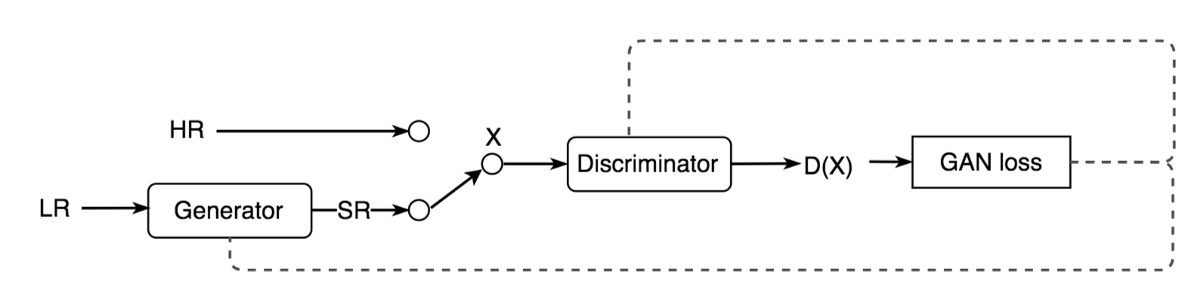
\includegraphics[width=6in]{Images/GANStructure.png}
				
				\texttt{Figure 1: GAN Model Structure}
				\vspace{0.1in}
			\end{center}
			
			In the previous cycle the GAN model learned, but to enhance the performance and the accuracy some blocks are added to make some balance in training process based on its skip connection for the network layers in between, that's in Generator part. And for more enhancement and go with the model deeper for better results, we combined residual blocks with each other to give Residual-In-Residual blocks (RIR Blocks). Will be discussed later in details.
			
			The Discriminator works as a closed component just to review Generator's results and decides whether each instance of data that it reviews belongs to the actual training dataset or not.
			
			Here are the base steps a GAN takes:
			\begin{enumerate}
				\item Generator takes in Low-Resolution image and returns a Super-Resolution image.
				\item Super-Resolution image is fed to the Discriminator alongside the actual High-Resolution image taken from the actual, ground-truth dataset.
				\item Discriminator takes in both real and fake images and returns probabilities, a number between 0 and 1, with 1 representing a prediction of authenticity and 0 representing fake.
				
				So, you have a double feedback loop:
				
				\item Discriminator is in a feedback loop with the ground truth of the images, which we know.
				\item Generator is in a feedback loop with the Discriminator.
			\end{enumerate}
			
			To sum up: \textsc{Generative Adversarial Networks} are neural networks that learn to choose samples from a special distribution (the \textsc{Generative} part of the name), and they do this by setting up a competition (hence \textsc{Adversarial}).
			
			A \textsc{Residual Block} is simply when the activation of a layer is fast-forwarded to a deeper layer in the neural network.
			\begin{center}
				\vspace{0.1in}
				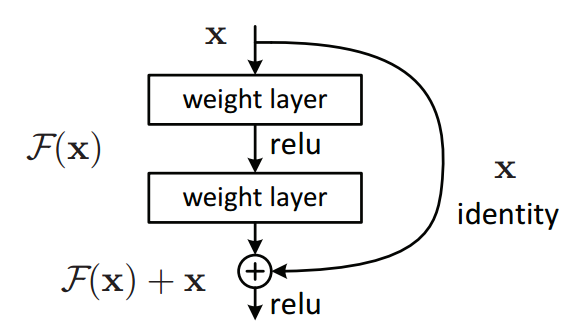
\includegraphics[width=4in]{Images/ResidualStructure.png}
				
				\texttt{Figure 2: Residual Block Structure}
				\vspace{0.1in}
			\end{center}
			
			As you can see in the image above, the activation from a previous layer is being added to the activation of a deeper layer in the network. This simple tweak allows training much deeper neural networks. In theory, the training error should monotonically decrease as more layers are added to a neural network. In practice however, for a traditional neural network, it will reach a point where the training error will start increasing. \textsc{ResNets} do not suffer from this problem. The training error will keep decreasing as more layers are added to the network. In fact, \textsc{ResNets} have made it possible to train networks with more than 100 layers, even reaching 1000 layers.
			
			We define a novel perceptual loss using high-level feature maps of the VGG network combined with a Discriminator that encourages solutions perceptually hard to distinguish from the HR reference images. An example photo-realistic image that was super resolved with a 4x up scaling factor.
		\subsection{Motivation}
			\textsc{Generative Adversarial Networks} have shown amazing image generative capabilities from the indoor scenes to the celebrity faces, super resolution can benefit from using the techniques from GANs. SISR has been used in many applications, such as:
			\begin{itemize}
				\item Optical Character Recognition (OCR).
				\item Face Recognition.
				\item Scene Detection.
				\item Satellite Image Processing
				\item Medical Image Processing.
				\item …etc.
			\end{itemize}
		\subsection{Problem Definition}
			To recover or restore High-Resolution image from Low-Resolution image. There are many forms of image enhancement which includes \textit{noise-reduction, image sharpening, up-scaling image, brightness} and \textit{colour adjustments}. This Project is based on enhancing Low-Resolution images by applying \textsc{Deep Network with Adversarial Network(Generative Adversarial Networks)} to produce High-Resolutions images.
			
			The target is to reconstruct Super-Resolution image or High-Resolution image by UpScaling Low-Resolution image such that texture detail in the reconstructed Super Resolution image is not lost.
		
	\clearpage
	\section{Literature Review and Related Work}
		\subsection{Introduction}
			\textsc{Super-Resolution Generative Adversarial Networks}(SRGAN) applies a deep network in combination with an \textsc{Adversary Network} to produce higher resolution images. SRGAN is more appealing to a human with more details compared with the similar design without GAN (SRResNet).
			
			In this section we review some existing Super-Resolution methods, some of which will be compared with the proposed method.
		\subsection{Literature Review}
			Many existing image Super-Resolution methods need multiple Low-Resolution images as inputs. We refer to them as \textsc{Multiple Image Super-Resolution}(MISR). Mathematically, there are $p$ Low-Resolution images $y_i\in{R^m}$ available, $y_i$ is related to a High-Resolution image $x\in{r^n}$ by $$y_i = DB_ix+n_i, 1\leq{i}\leq{p}$$ Where $D\in{R^{m*n}}$ is a down-sampling operator and $B_i\in{R^{n*n}}$ is a blurring operator that might happen due to for instance out of focus, $n_i\in{R^m}$ represents random noise.\cite{1}
			
			This project addresses \textsc{Single Image Super-Resolution}(SISR), i.e., $p = 1$. Compared to \textsc{Multiple Image Super-Resolution}(MISR), Single Image Super-Resolution is more applicable when there is only one Low-Resolution image available. Obviously, it is also more challenging.
			
			Existing Super-Resolution methods, for both multiple images and single image, can be roughly put into several categories: \textsc{Interpolation-Based}, \textsc{Statistics-Based}, \textsc{Learning-Based}, ...etc. This classification is by no means the best but provides an organized way for literature review. Note that, ideas of methods in different category might have overlap. For instance, some Learning-Based methods might also involve Statistics.
			
			\textsc{Interpolation} is a straightforward idea for image Super-Resolution. There are two popular classical interpolation methods: \textsc{Nearest-Neighbour Interpolation} and \textsc{Bicubic Interpolation}. Nearest-Neighbour Interpolation fills in intensity at an unknown location by that of its nearest neighbour point. It often causes jaggy effect, (Figure 3(c)). Bicubic Interpolation is to utilize a \textit{Cubic Kernel} to interpolate. It tends to create blur effect, (Figure 3(b)). Recently, some state-of-the-art interpolation methods have been proposed.
			\begin{center}
				\vspace{0.1in}
				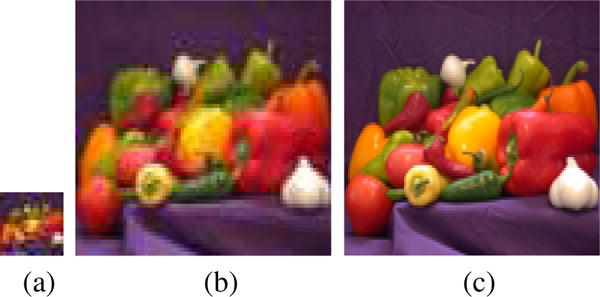
\includegraphics[width=6in]{Images/BiCubicVSNN.jpg}
				
				\texttt{Figure 3:(a)Low-Resolution;(b)Bicubic Interpolation;(c)Nearest Neighbour}
				\vspace{0.1in}
			\end{center}
			
			\textsc{Maximum a Posterior}(MAP) and \textsc{Maximum Likelihood Estimator}(MLE) are popular statistics-based methods \cite{2}\cite{3}. To preserve sharp edges, Fattal \cite{2} utilized statistical edge dependency to relate edge features in low and high-resolution images. Farsin et al. \cite{3} proposed an alternate approach using L1 norm minimization and a bilateral prior based robust regularization.
			
			\textsc{Learning-Based} approaches are a powerful tool for image Super-Resolution \cite{4}\cite{5}. They normally start from two large training data sets, one formed of Low-Resolution images and the other formed of High-Resolution images, and then learn a relation between Low-Resolution and High-Resolution images. The relation is then applied to a given Low-Resolution image to get a High-Resolution image. Learning-Based methods usually can obtain high quality images but they are computationally expensive. The results might depend on the selection of training data. Additionally, they are not a completely single image super-resolution since two large data sets are required for learning.
			
			In summary, \textsc{Single Image Super-Resolution}(SISR) is still a challenging problem. Existing single image super-resolution methods either need training data sets and expensive computation or lead to blur or jaggy effects.
		\subsection{Related Work}
			\subsubsection{Image Super-Resolution}
				Recent overview articles on image Super Resolution include Nasrollahiand Moeslund \cite{6} or Yang et al. \cite{7}. Here we will focus on \textsc{Single Image Super-Resolution}(SISR) and will not further discuss approaches that recover HR images from multiple images. \textit{Prediction-Based} methods were among the first methods to tackle SISR. While these filtering approaches. \textit{Linear}, \textit{Bicubic}, can be very fast, they oversimplify the SISR problem and usually yield solutions with overly smooth textures. Methods that put particularly focus on \textsc{Edge-Preservation} have been proposed \cite{8}. More powerful approaches aim to establish a complex mapping between Low and High-Resolution image information and usually rely on training data. Many methods that are based on \textsc{Example-Pairs} rely on LR training patches for which the corresponding HR counterparts are known. Early work was presented by Freeman et al. \cite{9}\cite{10}. In Glasner et al. \cite{11} the authors exploit \textsc{Patch Redundancies} across scales within the image to drive the SR. This paradigm of \textit{Self-Similarity} is also employed in Huanget al. \cite{12}, where \textsc{Self-Dictionaries} are extended by further allowing for small transformations and shape variations. To super-resolve landmark images, Yue et al. \cite{13} retrieve correlating HR images with similar content from the web and propose a structure-aware matching criterion for alignment. Neighbourhood embedding approaches up sample a LR image patch by finding similar LR training patches in a low dimensional manifold and combining their corresponding HR patches for reconstruction \cite{14}\cite{15}.
			\subsubsection{Convolutional Neural Networks}
				The \textsc{State of the Art} for many computer vision problems is meanwhile set by specifically designed CNN architectures following the success of the work by Krizhevsky et al. \cite{16}.It was shown that deeper network architectures can be difficult to train but have the potential to substantially increase the network’s accuracy as they allow multimappings of very high complexity \cite{17}\cite{18}.To efficiently train these deeper network architectures, \textsc{Batch-Normalization} \cite{19} is often used to counteract the internal covariate shift. Deeper network architectures have also been shown to increase performance for SISR, e.g. Kim etal. \cite{20} formulate a recursive CNN and present state-of-the-art results. Another powerful design choice that eases the training of deep CNNs is the recently introduced concept of \textsc{Residual Blocks} \cite{21} and \textsc{Skip-Connections} \cite{20}. Skip-Connections relieve the network architecture of modeling the identity mapping that is trivial in nature, however, potentially non-trivial to represent with convolutional kernels. In the context of SISR it was also shown that learning \textit{UpScaling} filters is beneficial in terms of accuracy and speed \cite{22}. This is an improvement over Dong et al. \cite{23} where \textit{Bicubic Interpolation} is employed to upscale the LR observation before feeding the image to the CNN.
			\subsubsection{Loss Function}
				\textbf{Pixel-Wise Loss} functions such as MSE struggle to handle the uncertainty inherent in recovering lost \textit{High-Frequency} details such as texture; minimizing MSE encourages finding Pixel-Wise averages of plausible solutions which are typically \textit{Overly-Smooth} and thus have poor perceptual quality. The \textsc{MSE-Based} solution appears overly smooth due to the Pixel-Wise average of possible solutions in the pixel space, while GAN drives the reconstruction towards the natural image manifold producing perceptually more convincing solutions.
				\begin{center}
					\vspace{0.1in}
					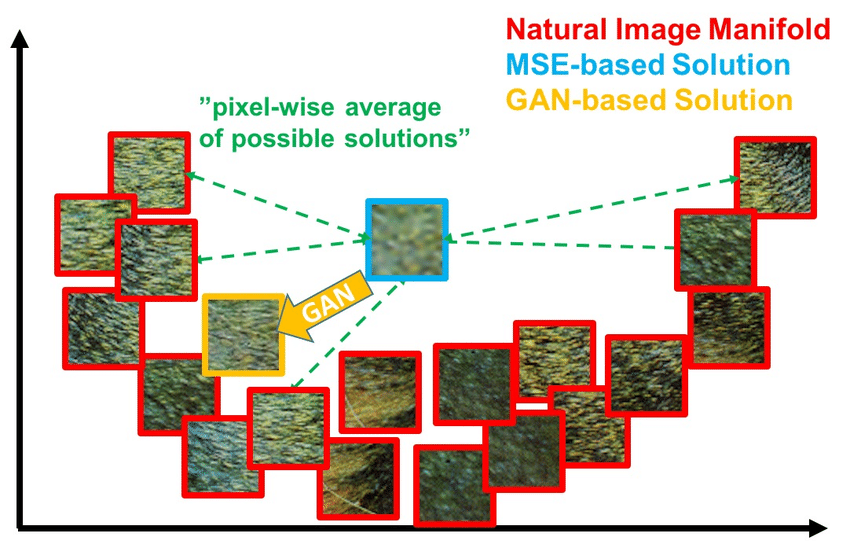
\includegraphics[width=6in]{Images/PW.png}
				
					\texttt{Figure 4: Illustration of patches from the natural image manifold (red)  and super-resolved patches obtained with MSE (blue) and GAN (orange).}
					\vspace{0.1in}
				\end{center}
			
				Multiple potential solutions with high texture details are averaged to create a smooth reconstruction. Yu and Porikli \cite{24} augment Pixel-Wise MSE loss with a discriminator loss to train a network that super-resolves face images with large UpScaling factors (8X). GANs were also used for \textit{Unsupervised Representation Learning} in Radford et al. \cite{25}. Dosovitskiy and Brox \cite{26} use loss functions based on Euclidean distances computed in the feature space of neural networks in combination with adversarial training. It is shown that the proposed loss allows visually better -In Some Cases- image generation and can be used to solve the ill-posed inverse problem of decoding nonlinear feature representations. Similar to this work, Johnson et al. \cite{27} propose the use of features extracted from a pre-trained VGG network instead of low-level pixel-wise error measures. Specifically, the authors formulate a loss function based on the Euclidean distance between feature maps extracted from the VGG19 \cite{17} network. Recently, Li and Wand \cite{28} also investigated the effect of comparing and blending patches in pixel or VGG feature space.
		\subsection{Conclusion}
			We have described a \textsc{Deep Residual Network In Conditional Adversarial Nets of the Generative Adversarial Networks} (GAN) model that sets a new state-of-the-art on public benchmark datasets when evaluated with the widely used PSNR measure. We have highlighted some limitations of this PSNR-Focused image Super-Resolution and introduced SRGAN, which augments the content loss function with an adversarial loss by training a GAN. We have confirmed that SRGAN reconstructions for small UpScaling factors (2x) are better than traditional image processing techniques and basic neural networks, but close and may be better than GAN models in some cases.
			
	\clearpage
	\section{SISR Using Residual Block in GAN Model}
		\subsection{Introduction}
			In this chapter, we present motivation and scope of a step forward in image enhancement carried out in this documentation. We also discuss the various applications of image super resolution that motivate us to work on this topic due to its large number of industry applications.
			\subsubsection{Background}
				\textsc{Super-Resolution} (SR) refers to the task of restoring High-Resolution images from one or more Low-Resolution observations of the same scene. According to the number of inputs LR images, the SR can be classified into \textsc{Single Image Super-Resolution} (SISR) and \textsc{Multiple Image Super-Resolution} (MISR). Compared with MISR, SISR is much more popular because of its high efficiency. Since an HR image with high \textit{Perceptual Quality} has more valuable details, it is widely useful in many areas, such as \textit{Medical Imaging}, \textit{Satellite Imaging} and \textit{Security Imaging}. In the typical SISR framework.
			\subsubsection{Scope}
				It is investigated that \textsc{Super Resolution Reconstruction Techniques} are still under development. All the existing methods of Super-Resolution reconstruction do not provide satisfactory results; therefore, it is required to investigate the better model which provides the better accuracy. High-Resolution images require higher storage, it is beneficial to store the images in Low-Resolution and construct the HR images whenever required from Low-Resolution images. In addition, High-Resolution images contain more details and information about the image and have less noise.
				
				\textsc{Low-Resolution} (LR) image has small pixel density within an image, therefore offers fewer details. \textsc{High-Resolution} (HR) image has larger pixel density within an image, therefore offering more details. \textsc{Super-Resolution} (SR) can be obtained from one or multiple LR images. The important question is: \textbf{How to Increase Resolution?} Possible ways for increasing an image resolution are reduce \textit{Pixel Size}; Increase the \textit{Chip-Size} and \textit{Super-Resolution}. By reducing pixel size, the number of pixels per unit area will increase. The disadvantage is noise introduced and the pixel size decreases, the amount of light decreases. Next, to increase the Chip-Size (HW), it enhances spatial resolution but high cost for high precision optics.
				
				Now-A-Days, \textsc{High Resolution} images are widely used in most of the image processing applications such as \textit{Remote Surveillance}, \textit{Video Enhancement}, \textit{Industrial Inspection},\textit{Medical Imaging}, \textit{Robot Vision} and \textit{Remote Sensing}. Firstly, the idea of Super-Resolution was introduced by Tsai and Huang (1984) using the frequency domain approach. Processing power limitations and channel capabilities are some factors which make the images to be transmitted at low bit rates and often down sampled which results in a Low-Resolution compressed image. Super-Resolution is the technique of producing a higher \textsc{Spatial Resolution} image from one or more such under sampled Low-Resolution images, Low-Resolution refers to the less pixel density in an image which offers very few details.
				
				\textbf{PSNR} is one of the most common \textsc{Quantitative Parameters} used to measure validity of the SR methods. But practically higher solution image is unknown. So, an alternate parameter should be developed to check the quality of Super-Resolved image. It will also be interesting to develop a mathematical model for Learning-Based Super-Resolution techniques.
		\subsection{Proposed System}
			In SISR the aim is to estimate a High-Resolution, Super-Resolved image $I^{SR}$ from a Low-Resolution input image $I^{LR}$. Here $I^{LR}$ is the Low-Resolution version of its High-Resolution counterpart $I^{HR}$. The High-Resolution images are only available during training.
			
			Before training, a \textsc{Pre-Processing} stage is applied on the $I^{HR}$ images, the $I^{LR}$ is obtained from the $I^{HR}$ images by down-sizing it with \textsc{Bicubic Interpolation}. Our training dataset is the DIV2k dataset \cite{29} which contains 900 training images, beside to cropping the whole images into small squared images with different sizes to be the total number of $I^{HR}$ dataset. Then split the data by 9:1 for training and testing respectively. In both phases training and testing we standardize any image with a \textsc{Normalization} for faster processing and after the last step we do \textsc{De-Normalization} the image again to original.
			
			As we mentioned before, The GAN consists of two basic components. the first component is \textsc{Generator}, which has the most important role in generating and building new pixels in a LR input image. The second component is \textsc{Discriminator} which reviews on what the generator has generated and give a loss and some edits that is based on them the generator will improve its output.
			
			The general idea behind this formulation is that it allows one to train a generative model with the goal of fooling a differentiable discriminator model that is trained to distinguish Super-Resolved images from real images. With this approach our generator can learn to create solutions that are highly similar to real images and thus difficult to classify by discriminator.
			
			\subsubsection{Discriminator Model}
				We use a Discriminator to distinguish the High-Resolution HR images and Back-Propagate the GAN loss to train the Discriminator and the Generator. Our proposed discriminator life cycle is as follow:
				\begin{itemize}
					\item We create the \textsc{Discriminator Base Block (DBB)} which consists of three layers (\textit{Conv2D}, \textit{LeakyReLU} and \textit{Batch Normalization}).
					\item The full Discriminator Block mainly consists of 8 DBB with respect of different filters number and \textit{Padding “same”} in every \textit{Conv2D} layer, A \textit{Flatten}, \textit{Dense}, \textit{LeakyReLU} and \textit{Dens} layers are added to the end of the model.
					\item It uses \textsc{Adam Optimizer} and \textsc{Binary Cross Entropy} in loss.
					\item It is not trainable during the full GAN training.
					\item It is trainable during updating discriminator training on the $I^{HR}$ and the $I^{SR}$ to distinguish between them and be able to provide the generator with better feature details.
				\end{itemize}
				\begin{center}
					\vspace{0.1in}
					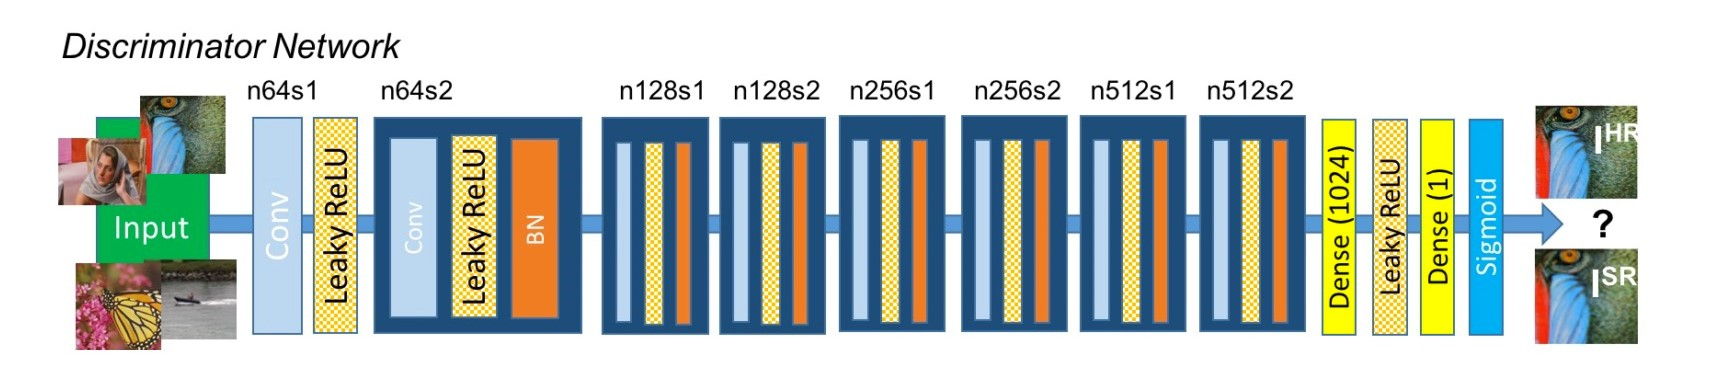
\includegraphics[width=6in]{Images/Discriminator.jpeg}
				
					\texttt{Figure 5: Discriminator Model Architecture.}
					\vspace{0.1in}
				\end{center}

			\subsubsection{Generator Model}
				As described earlier, the \textsc{Generator} is a function that transforms a random input into a synthetic output. In GAN Lab, a random input is a 2D sample with a (x, y) value, and the output is also a 2D sample, but mapped into a different position, which is a fake sample. We used \textsc{Residual Blocks} with the respect of the advantage of \textsc{Skip Connections} which keeps more feature and information from the Skip Connection start layer.
					
				Our \textsc{Residual Blocks} is overall trying to learn the true output, you can skip the training of few layers using \textsc{Skip Connections} or \textsc{Residual Connections}. It has also been observed that it is easier to learn residual of output and input, rather than only the input. As an added advantage, our network can now learn \textit{Identity Function} by simply setting residual as zero. And if you truly understand \textsc{Back-Propagation} and how severe the problem of \textsc{Vanishing Gradient} becomes with increasing number of layers, then you can clearly see that because of these skip connections, we can propagate larger gradients to initial layers and these layers also could learn as fast as the final layers, giving us the ability to train deeper networks.
					
				We enhanced the well-known GAN models with the \textsc{Residual Blocks}. We created our own block with respect of the added residuals and skip connections between each block (not to forget the already added skip connection built in between every residual blocks). Our blocks can have multiple residual blocks as many as you require for the application, which will -hopefully- improve the accuracy of your model, it is also can be used in any different kind of models, not just the GAN models. In our tesing and validating the performance of our idea, We built our generator by adding six RIR Blocks which contain three residual blocks in each. Our proposed generator life cycle:
				\begin{itemize}
					\item \textsc{Normalization} is added to the model to help in speeding processing time, with respect of \textsc{De-Normalization} at the end.
					\item The model starts with basic \textit{Conv2D} and \textit{PReLU} layers.
					\item We save our main skip connection which will be passed to the end of the model skipping all the RIR blocks.
					\item We add the \textsc{RIR Blocks} with respect of saving and adding the skip connection on every RIR block.
					\item The \textsc{RIR Block} is built using multiple \textsc{Residual Blocks} and its \textsc{Skip Connections}.
					\item After adding the \textsc{RIR Blocks} with its \textsc{Skip Connection}, we add all the \textit{Skip Connections}, \textit{Conv2D} and \textit{PReLU} layers.
					\item The \textsc{UpSampling} phase is now on. We add UpSampling Blocks based on the scaling factor based on the $I^{HR}$ and $I^{LR}$ ratio.
					\item \textsc{De-Normalization} After UpSampling block to recover original pixels values of image.
				\end{itemize}
				\begin{center}
					\vspace{0.1in}
					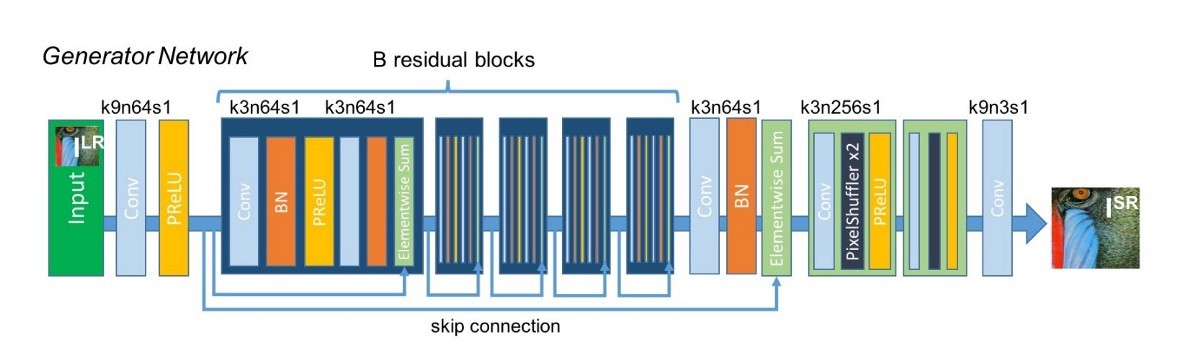
\includegraphics[width=6in]{Images/Generator.jpeg}
				
					\texttt{Figure 6: Generator Model Architecture.}
					\vspace{0.1in}
				\end{center}
			\subsubsection{Full GAN Model}
				Here is connection between the \textsc{Generator} and the \textsc{Discriminator} to produce a GAN model is created. The GAN starts with the Generator input image $I^{LR}$, then the generated image $I^{SR}$ is passed as a fake image to the Discriminator along-side with the real image $I^{HR}$.
				
				We used \textsc{Adam Optimizer} for the optimization of the loss function of the full GAN model.
				
				Our loss function is based on the pre-trained \textsc{VGG19} model, which is trained on ImageNet database. The network is 19 layers deep and can classify images into 1000 object categories, such as keyboard, mouse, pencil, and many animals. As a result, the network has learned rich feature representations for a wide range of images. The VGG loss function works as followed:
				\begin{itemize}
					\item Extract $I^{SR}$ features.
					\item Extracts $I^{HR}$ features.
					\item Calculate the \textsc{Mean Squared Error} (MSE).
				\end{itemize}
			
			\subsubsection{GAN Model Training}
				As we mentioned before, the dataset get through pre-processing which gives us different number of images for each resolution.
				\begin{center}
					\vspace{0.4in}
					\begin{tabular}{c|c|c|c}
						\textbf{Training $I^{HR}$ Resolution} & \textbf{256*256} & \textbf{128*128} & \textbf{96*96} \\\hline
						\textbf{Images Count} & 31,101 & 136,110 & 263,298\\\hline
						\textbf{Cropping Time(minutes)} & 2:26 & 3:43 & 5:31
					\end{tabular}
					\vspace{0.2in}
					
					\texttt{Table 1: Datset Size for each Resolution.}
					\vspace{0.1in}
				\end{center}
				
				Images are split by 9:1 for training and testing respectively.
				
				For each training batch we do the followed:
				\begin{itemize}
					\item Get a random sample of training images ($I^{LR}$ and its $I^{HR}$) with the limit of batch size.
					\item Pass $I^{LR}$ to generator model to predict $I^{SR}$.
					\item Discriminator is now set as trainable.
					\item Pass $I^{SR}$ and its $I^{HR}$ to Discriminator model to train on distinguishing between real and fake images.
					\item Discriminator is now set as not-trainable.
					\item GAN model is set on training.
				\end{itemize}
				
				For each epoch we do model evaluation on test dataset of all $I^{LR}$ and its generated $I^{SR}$ from generator:
				\begin{itemize}
					\item Calculating the total averages of \textsc{Peak-To-Noise-Signal-Ratio}. (PSNR).
					\item Calculating the total averages of \textsc{Structural Similarity Index} (SSIM).
					\item Calculating the total averages \textsc{Mean Squared Error} (MSE).
				\end{itemize}
	
	\clearpage
	\section{Software Requirements Specifications}
		\subsection{Introduction}
			This chapter contains the system requirements for our project. It includes includes descriptions of the Functions, the Specifications of the project, Software and Hardware constrains.
			\subsubsection{Purpose}
				The core goal here is to ease using our GAN model by build a web application which allow user to upload a Low-Resolution image and get a new generated one with a higher resolution and more details.
			\subsubsection{Scope}
				Now-A-Days, \textsc{High Resolution} images are widely used in most of the image processing applications such as \textit{Remote Surveillance}, \textit{Video Enhancement}, \textit{Industrial Inspection},\textit{Medical Imaging}, \textit{Robot Vision} and \textit{Remote Sensing}.
				
				So, our \textsc{Web Application} is to cover non-technical users' needs by perform our model on his uploaded Low-Resolution image and reconstruct a new Super-Resolution image. After the training and testing phases of our model, we must deploy this trained model on server and connect it with the implemented web application.
			\subsubsection{Overview}
				Now, we can say that this project consists of two different parts: Deep Learning (Model) and the other part is Web Application part for usability and to make the model user friendly not just command lines and technical details.
				
				The core value of this project is to UpScale the Low-Resolution images to Super-Resolution images based on a Deep Learning approach, \textsc{Conditional Adversarial Nets of the Generative Adversarial Networks (GAN) Model}. The first component is Generator, which has the most important role in generating and building new pixels from a LR input image. The second component is Discriminator which reviews on what the generator has generated and give a loss and some edits that is based on them the generator will improve its output in next iteration.
				
				After that, it’s necessary to deploy our model in an app for any use. Here, we build out web application using React and Python. React usually used for front end process like Upload and Display image to make a user interface be able to use the deep learning model. Python is used to create a server to handle the uploaded images and to enhance the image using the pre-trained model. Return the enhanced images to the React app to display them. This tool also used to save image on server, send it to UI to display and handling time clock issues like synchronization.
		\subsection{General Description}
			\subsubsection{Product Functions}
				Our implementation was in Python for the Deep Learning model, React and JavaScript for the Web Application.
				
				The basic functions of the GAN model in Python:
				\begin{itemize}
					\item Pre-Processing: Perform data preparation for training.
					\item BuildGenerator: Build Generator model layers with specified \textit{nRIR Blocks} and \textit{nResidual Blocks in RIR Block}.
					\item Generator: Generate the new Super-Resolution image from Low-Resolution image.
					\item BuildDiscrimitator: Build Discriminator model with specified input shape.
					\item Discriminator: Evaluate Generator output and guide it to edits.
					\item Train: Start training with specified attributes. e.g. \textit{Batch Size}, \textit{nRIR Blocks}, \textit{nResidual Blocks in RIR Block}, ...etc.
					\item ContentLoss: How is my output far from real (Loss function).
					\item Evaluation: Calculate the accuracy of testing image in different measures. 
				\end{itemize}
				
				The basic functions of Web Application in React and Python Server:
				\begin{itemize}
					\item React\\
						Used to make a \textit{User Interface} to be able to use the machine learning model with ease.
						\begin{enumerate}
							\item Upload image to be enhanced.
							\item Display enhanced Images.
						\end{enumerate}
					\item Python\\
						Used to create the server to handle the uploaded images and to apply the pre-trained model to enhance the image.
						\begin{enumerate}
							\item Save the uploaded image to be enhanced and use both Bicubic and our model to enhance it separately.
							\item Return the enhanced images to the React app to display them.
						\end{enumerate}
				\end{itemize}
			\subsubsection{Similar System Information}
				\textbf{SISR Using Skip Connection Deep CNN and Network in Network} (DCSCN)\cite{30} is a \textit{Fully Convolutional Neural Network}. As shown in Figure 5, DCSCN consists of a \textit{Feature Extraction Network} and a \textit{Reconstruction Network}. Cascaded a set of CNN weights, biases and non-linear layers to the input. Then, to extract both the local and the global image features, all outputs of the hidden layers are connected to the Reconstruction Network as Skip Connection. After concatenating all of the features, parallelized CNNs (Network in Network) are used to reconstruct the image details. The last CNN layer outputs the 4CH (or the channels of square of scale factor) image and finally the Up-Sampled original image is estimated by adding these outputs to the Up-Sampled image constructed by Bicubic Interpolation. Thus the proposed CNN model focuses on learning the residuals between the bicubic interpolation of the LR image and the HR original image.
				
				This proposed method is a fast and accurate Image Super Resolution method based on 	CNN with skip connection and network in network. In the feature extraction network of, the structure is optimized and both local and global features are sent to the	reconstruction network by skip connection. In the reconstruction network, network in network architecture is used to obtain a better reconstruction performance with less computation. In addition, the model is designed to be capable of processing original size images. Using these devices, the model can achieve state-of-the-art performance	with less computation resources.
			\subsubsection{User Characteristics}
				The main purpose of our system is to reconstruct High-Resolution image from ower version, using the system doesn’t require any special knowledge, just using the user interface in the web application.
			\subsubsection{User Objectives}
				\textbf{Super-Resolution} (SR) Refers to the task of restoring a High-Resolution images from one or more Low-Resolution observations from the same scene since $I^{HR}$ with high perceptual quality has more valuable details restoring a HR version can be such a difficult and slow task for humans to do manually it could take very long time and such a great effort. Single Image Super Resolution (SISR) is popular because of its high efficiency and its time utilization.
			\subsubsection{General Constraints}
				Based on our project, it’s obvious that the most important thing is the training images, size, colours and the huge number of contained details of training data all of them influence in output image for sure. So, there are a minimum requirement for the used device to build model and train it, we talk about RAM, CPU and specially GPU. But for using the final trained model on the web application with no problem, the application is hosted on a remote server connected with a stable Internet connection.
				\begin{itemize}
					\item GANs can be very difficult to train. Network can be very deep sometimes, but use of residual blocks makes it easier.
					\item It’s better to use images of the width and height other wise to have to do pre-processing to images to have them equally sized.
					\item A GPU to training is a must otherwise it would take months to train.
				\end{itemize}
		\clearpage
		\subsection{Functional Requirements}
			\begin{longtable}{|c|p{.8\textwidth}|c|}
				\hline
				\textbf{Req.} & \textbf{Description} & \textbf{Priority} \\
				\hline
				\textbf{FR1} & \textbf{User interaction with the application server:}
				\begin{itemize}
					\item User Interface is a gate for any user get use our model through a web application.
					\item First, User chooses an image file with any size to upload it to the wep application. It’s the Low-Resolution image.
					\item Second, the app front-end creates a request to the server side and pass the image.
					\item Third, validate the image and server back-end save it on the hosting server.
				\end{itemize} & HIGH \\
				\hline
				\textbf{FR2} & \textbf{Web Application Server requests Bicubic algorithm image generation from the remote Python server:}
				\begin{itemize}
					\item After the request that is created by web application server in \textit{FR1} to the Python server.
					\item First, Pass the uploaded image to the python server, to save it.
					\item Second, Re-Sizing starts on the save image.
					\item Third, Python server replies to the web application server's request by the enhanced image by the Bicubic algorithm.
				\end{itemize} & Medium \\
				\hline
				\textbf{FR3} & \textbf{Web Application Server request using GAN model from the remote Python server:}
				\begin{itemize}
					\item After the request that is created by web application server in \textit{FR1} to the Python server.
					\item First, Pass the uploaded image to the python server, to save it.
					\item Second, GAN model starts predicting the High-Resolution for the saved image.
					\item Third, Python server replies to the web application server's request by the enhanced image by the GAN model.
				\end{itemize} & Medium \\
				\hline
				\textbf{FR4} & \textbf{Collect Python server's response and display the result with a download option.}
				\begin{itemize}
					\item After receiving the responses from the Python server form the Bicubic algorithm and GAN model from FR2, FR3 returns.
					\item First, Back-End server passes the results to the Front-End application.
					\item Second, Front-End application displays the two Super-Resolution generated images in the UI.
					\item Third, The two Super-Resolution images are displayed, there is an option to download and zoom in-out the output generated images.
				\end{itemize} & Medium \\
				\hline
			\end{longtable}
		\subsection{Interface Requirements}
			\subsubsection{User interface}
				It’s a simple web page and easy to use by any user. It’s split into three equal parts:
				\begin{enumerate}
					\item Select image and upload it to the app server, then display it.
					\item Display the output of Bicubic interpolation algorithm.
					\item Display the output of out GAN model.
				\end{enumerate}
				
				Each part of them contains bars for zooming and scrolling to distinguish the differences and reset button to clear these boxes and wait a new image to show.
		\subsection{Performance Requirements}
			\subsubsection{Response Time}
				To prepare the training data or make out pre-processing for the model, the used time for cropping and saving the images for each resolution from the 900 images in \textbf{DIV2K} \cite{29} dataset is shown in (Table 1).
				
				To train our model and save the final weight matrix it costs us different average time for each epoch due to the model layers sizie and the amount of processing time in the training.
				\begin{center}
					\vspace{0.4in}
					\begin{tabular}{c|c|c|c|c}
						\textbf{Training $I^{HR}$ Resolution} & X & \textbf{256*256} & \textbf{128*128} & \textbf{96*96} \\\hline
						\multirow{2}{*}{\textbf{Total Params}} & 2x & 141,944,388 & 41,281,092 & 26,601,028 \\\cline{2-5} & 4x & 142,092,164 & 41,428,868 & 26,748,804\\\hline
						\multirow{2}{*}{\textbf{Trainable Params}} & 2x & 1,551,235 & 1,551,235 & 1,551,235 \\\cline{2-5} & 4x & 1,699,011 & 1,699,011 & 1,699,011\\\hline
						\multirow{2}{*}{\textbf{Non-Trainable Params}} & 2x & 140,393,153 & 39,729,857 & 25,049,793 \\\cline{2-5} & 4x & 140,393,153 & 39,729,857 & 25,049,793\\\hline
						\multirow{2}{*}{\textbf{Training Time(minutes/epoch)}} & 2x & -- & 64 & 80 \\\cline{2-5} & 4x & 7 & 50 & 75
					\end{tabular}
					\vspace{0.2in}
					
					\texttt{Table 2: Training Comparison between different resolutions.}
					\vspace{0.1in}
				\end{center}
				
				To use and test the model in the web app it cost about two minutes as maximum and that’s based on the uploaded image to enhance and display it in two forms the Bicubic output and GAN output.
				
				Best saved model of each resolution and scale factor is tested on 500 images from the Flickr2K dataset \cite{31}, the test results is in (Table 3).
			\subsubsection{Resources}
				We trained our model on DIV2K \cite{29} dataset, It’s a \textit{Benchmark Dataset} and totally free. The training machine should have a solid GPU with respectful memory to be able to load the memory and train it, if you thought in training with using only the CPU, it would take forever specially if you want to train for a huge number of epochs. For GPUs, we thought of training with \textit{GTX 1060 6 GB}, but we got into \textsc{Memory Limit Failing} due to the model size which can't be fit in the 6 GB VRAM. We need to get more VRAM, so we went with \textit{GTX 1080ti 11 GB}, it was very convenient and almost enough for our tests. To be clear, we couldn't go beyond HR of 256 because of memory limit.
				
				For the training we used a powerful machine with solid performance:
				\begin{itemize}
					\item \textbf{RAM}: 16 GB
					\item \textbf{CPU}: Intel Core i7-8700
					\item \textbf{GPU}: Nvidia GTX 1080ti, 11 GB VRAM
				\end{itemize}
				
				For remote hosting server for the Python Server on Digital Ocean, we used these specifications:
				\begin{itemize}
					\item \textbf{CPU}: 4 vCPUs
					\item \textbf{RAM}: 8 GB
					\item \textbf{Hard Disk}: 25 GB
				\end{itemize}
		\subsection{Design Constraints}
			\subsubsection{Software}
				In the Deep Learning model training part, we are using different Python libraries to make this project possible, such as:
				\begin{itemize}
					\item CV2
					\item Keras
						\begin{itemize}
							\item Applications.VGG19
							\item Loses
							\item Models
							\item Layers
							\item Utils
							\item Optimizers
						\end{itemize}
					\item Numpy
					\item Skimage
					\item Tensorflow
					\item Matplotlib 
				\end{itemize}
				And for building the web application:
				\begin{itemize}
					\item React
					\item Node.js
				\end{itemize}
			\subsubsection{Hardware}
				Based on our test, the recommended machine for training preferred to have these specifications:
				\begin{itemize}
					\item \textbf{RAM}: 16 GB
					\item \textbf{CPU}: Intel Core i7-8700
					\item \textbf{GPU}: Nvidia Tesla V100, 32 GB VRAM
				\end{itemize}
				
				For remote hosting server for the Python Server on Digital Ocean, we used these specifications:
				\begin{itemize}
					\item \textbf{CPU}: 4 vCPUs
					\item \textbf{RAM}: 8 GB
					\item \textbf{Hard Disk}: 25 GB
				\end{itemize}
				It might be a good addition to have also a decent GPU for the Web Application.
		\subsection{Other Non-Functional Requirements}
			\subsubsection{Usability}
				\textbf{Definition}: The degree to which a software can be used by specified consumers to achieve quantified objectives with \textit{effectiveness}, \textit{efficiency}, and \textit{satisfaction} in a quantified context of use.
				
				The web interface that the system had works as a \textit{Website} for the user to use our application correctly without a need for learning specific skill or special operation. All the user need is to follow those steps to get the right output from the application:
				\begin{itemize}
					\item Upload Low-Resolution photo using the website.
					\item The application's Back-End server will process your photo using our pre-trained model.
					\item The user will get the Super-Resolution image processed and ready to be downloaded.
				\end{itemize}
				
				\textbf{Efficiency of Use}: The average time it takes to accomplish a user's goals. Just couple of seconds by uploading the image that needed to be enhanced. The tasks that user can complete without any interruption are uploading the Low-Resolution image and downloading the Super-Resolution one.
				
				\textbf{Intuitiveness}: It is easy to understand the interface, all the user need to get familiar with is the interface by using just two buttons \textit{Upload} and \textit{Download} buttons.
				
				\textbf{Low Perceived Workload}: The user need just two attempts to accomplish the whole task which is enhance the resolution of a single Low-Resolution image.
			\subsubsection{Reliability}
				\textbf{Definition}: Is how likely it is for the software to work without failure for a given period of time. Reliability decreases because of \textit{Bugs in the Code}, \textit{Hardware Failures}, or \textit{Problems with other System Components}. To measure software reliability, you can count the percentage of operations that are completed correctly or track the average period of time the system runs before failing.
				
				Our Application have a good structure that relay on, though the system works well under the normal requests pressure, the system can handle various user's requests at the same time without suffering from errors.
				
				The user send request to get the Low-Resolution image enhanced by uploading the desired image and the system will response with the Super-Resolution image, this process can by performed by multiple users at the same time using the system's web interface normally.
			\subsubsection{Maintainability}
				\textbf{Definition}: Is the ease with which an application can be maintained to \textit{Correct Defects or their cause}, \textit{Maximize Efficiency}, \textit{Reliability}, and \textit{Safety} meet new requirements, maximize a product's useful life or it can be defined as degree of effectiveness and efficiency with which a system can be modified by the intended maintainers.
				
				The whole Application is maintainable as we can update some functionality to make the user experience better and handle the errors that might be barrier for the user.
			\subsubsection{Portability}
				\textbf{Definition}: Is the usability of the same software in \textit{Different Environments}, how the user can access this software from \textit{Various Platforms}.
				
				The user can access the application from various platform as the application has a web interface that the user can get to it using Mobile phones or any laptops All the user need is to access to the internet to access the application.
			\subsubsection{Security}
				\textbf{Definition}: Is the degree to which application protects information and data so that persons or other products or applications have the degree of data access appropriate to their types and levels of authorization.
				
				Our application is securing the user data, every user has his own session on the web interface of the application so the user data can't be accessed by another, the application just dealing with images format of the data so the user can't upload any other files to the system.
			\subsubsection{Availability}
				\textbf{Definition}: Is the degree to which a system, product or component is \textit{Operational} and \textit{Accessible} when required for use. 
				
				Our application is available to be used when the user need (on demand), the application has a web interface that makes the accessibility and availability very easy.
		\subsection{Object Oriented Domain Analysis}
			\begin{center}
				\vspace{0.1in}
				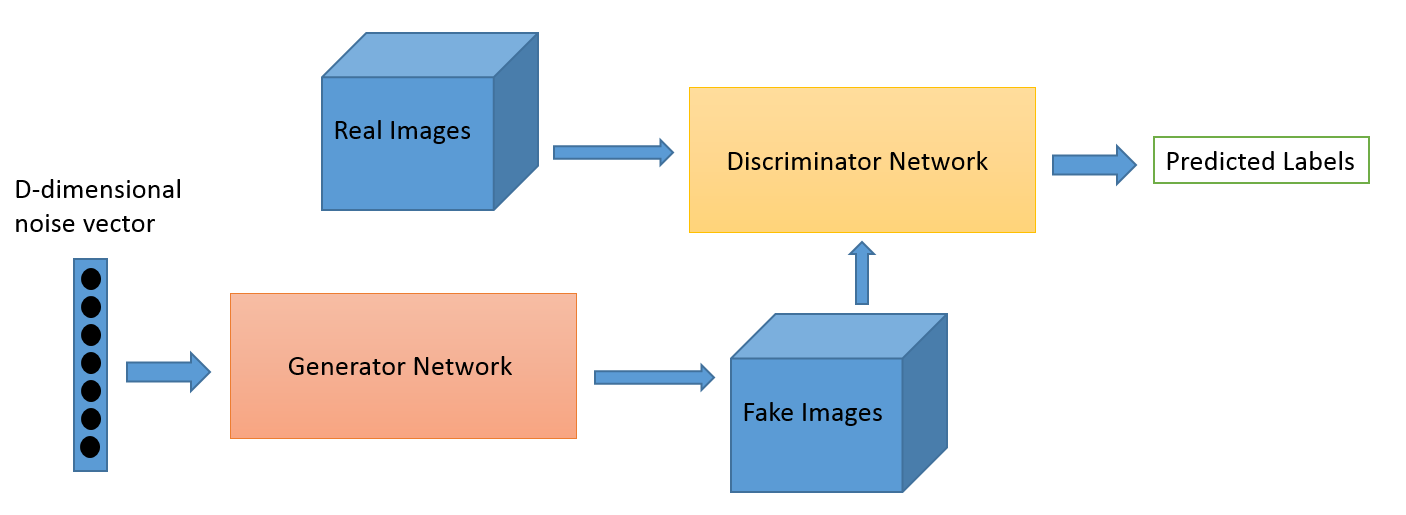
\includegraphics[width=6in]{Images/GANBlockDiagram.png}
				
				\texttt{Figure 7: Relation Between G \& D in a Block Diagram}
				\vspace{0.1in}
			\end{center}
			Our OO Classes will be discuss in this section. We created three main classes:
			\begin{itemize}
				\item Generator
				\item Discriminator
				\item GAN
			\end{itemize}
			
			As we explained before that any GAN implementation must include the two basic components: \textit{Generator} and \textit{Discriminator}. The dependency of GAN class on the Generator and Discriminator classes is very high so the relation between GAN and them is a composition relation. Without Generator or Discriminator there will be no GAN.
			
			\begin{center}
				\vspace{0.1in}
				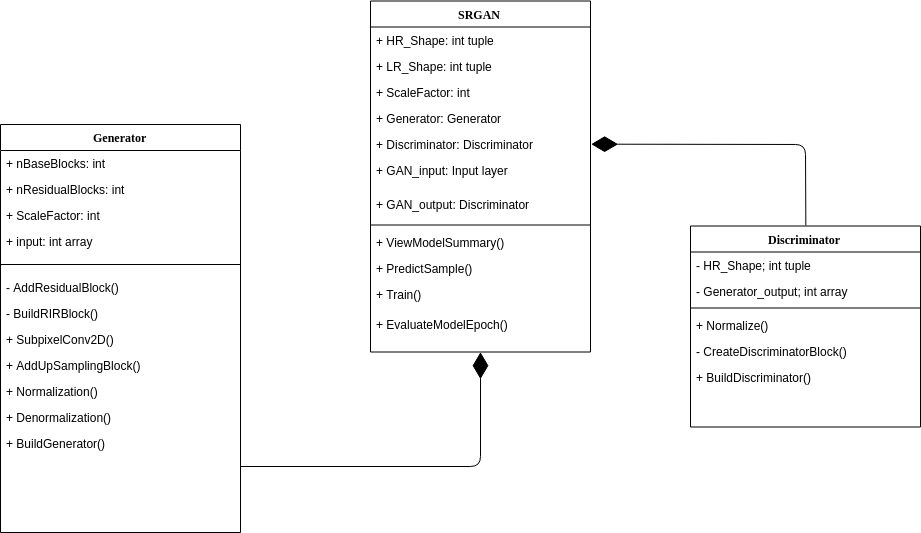
\includegraphics[width=6in]{Images/ClassDiagram.png}
				
				\texttt{Figure 8: GAN Class Diagram}
				\vspace{0.1in}
			\end{center}
			The \textsc{Class Diagram} describes the relation in more details:
			\begin{itemize}
				\item \textbf{Generator} is built to generates the Super-Resolution output image based on the input Low-Resolution image, using these functions:
					\begin{itemize}
						\item \textbf{init}: Object class initializer.
						\item \textbf{AddResidualBlock}: Create one residual block and add it to the model.
						\item \textbf{BuildRIRBlock}: Calls AddResidualBlock function to build our enhanced architecture with \textit{Residual In Residual} blocks and nested skip connections.
						\item \textbf{SubpixelConv2D}: Get calculations from depth to prepare the new generated pixels.
						\item \textbf{AddUpSamplingBlock}: Create \textit{Up-Sampling} Block layers.
						\item \textbf{Normalization}: Re-Scale the pixels values of the input images and standardize them.
						\item \textbf{Denormalization}: Recover the original image from normalized image.
						\item \textbf{BuildGenerator}: Use all previous function to get the Generator model.
					\end{itemize}
				\item \textbf{Discriminator} reviews on the generator output and evaluates the losses based on output, using these functions:
					\begin{itemize}
						\item \textbf{init}: Object class initializer.
						\item \textbf{Normalize}: Re-Scale the pixels values of the input images and standardize them.
						\item \textbf{CreateDiscriminatorBlock}: Builds the \textit{Base-Block} of Discriminator.
						\item \textbf{BuildDiscriminator}: Build Discriminator's layers by using the \textit{CreateDiscriminatorBlock} many times.
					\end{itemize}
				\item \textbf{SRGAN} is the main class that combines Generator and Discriminator models and starts training then starts evaluate it by a testing phase, using these functions:
					\begin{itemize}
						\item \textbf{init}: Object class initializer, Uses instance of Generator, Discriminator and AdamOptimizer to build the Full GAN model.
						\item \textbf{ViewModelSummary}: view a detailed summary about the model parameters and layers.
						\item \textbf{PredictSample}: Save a random sample contains three images: High-Resolution, Low-Resolution and the model output in a separated folder for each epoch.
						\item \textbf{Train}: Takes Low-Resolution images, High-Resolution images, Batch Size, Epochs Number and the path to save model progress, losses and its weights, then pass LR images to Generator class to train it on generating and pass HR images to Discriminator to train how to review Generator output.
						\item \textbf{EvaluateModelEpoch}: Calculates the average of these measures: PSNR, SSIM and MSE for output accuracy evaluation after each epoch training.
					\end{itemize}
			\end{itemize}
		\subsection{Operational Scenarios}
			\subsubsection{Use Case Diagram}
				\textsc{Use Case Diagram} is a dynamic or behavior diagram in UML. Use Case Diagrams model the functionality of a system using actors and use cases. Use cases are a set of \textit{Actions}, \textit{Services}, and \textit{Functions} that the application needs to perform. In this context, an "Application" is something being developed or operated, such as a Web-Site. The "Actors" are the people or entities operating under defined roles within the system.
				
				Our project application contains just \textit{One Actor} called User, \textit{Three Objects} or UI entities, \textit{App Server} and \textit{Model Server}. User selects an image want to be enhanced it to Super-Resolution, then Front-End UI receive it and pass it to Back-End model server which call the pre-trained model and apply the Bicubic algorithm on the sent image, then wait the output for the uploaded image.
				\begin{center}
					\vspace{0.1in}
					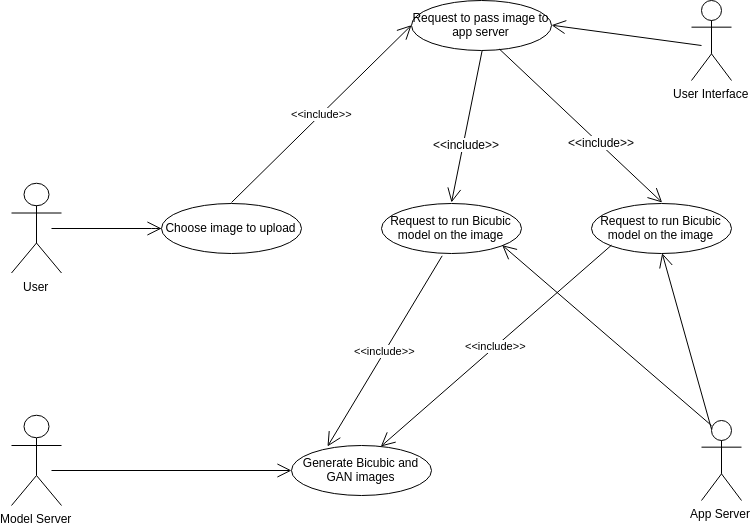
\includegraphics[width=6in]{Images/UseCaseDiagram.png}
				
					\texttt{Figure 9: Application Use Case Diagram}
					\vspace{0.1in}
				\end{center}
			
			\subsubsection{Sequence Diagram}
				\textsc{Sequence Diagram} is the \textit{Interaction Diagrams} that details how operations are carried out. They capture the interaction between objects in the context of a collaboration. Sequence Diagrams are time focus and they show the order of the interaction visually by using the vertical axis of the diagram to represent time what messages are sent and when.
				
				Here in this section is a listing of the same activities as messages by the take care of timing:
				\begin{itemize}
					\item Select an image to upload.
					\item UI Front-End server connects to Back-End server.
					\item Pass the image to the Back-End server.
					\item Back-End server saves the image.
					\item Back-End makes two operations:
						\begin{itemize}
							\item Pass the uploaded image to GAN model.
							\item Pass the same image to Bicubic algorithm.
						\end{itemize}
					\item Here, there is a synchronization in Front-End server to handle Back-End server returns.
					\item Display the two outputs.
					\item After all of that, there an optional message for the user to send, it's to download these generated output.
				\end{itemize}
			\subsubsection{Activity Diagram}
				\textsc{Activity Diagram} is basically a flowchart to represent the flow from one activity to another activity. The activity can be described as an operation of the system. 
				
				As we mention before, that the application works as followed:
				\begin{itemize}
					\item Choose an image to upload.
					\item Fron-End server sends image to Back-End server.
					\item Back-End receives image and start applying \textit{Bicubic Algorithm} and user the \textit{Pre-Trained GAN Model}.
					\item The Back-End server send the request replay with the processed images to the Fron-End server.
					\item Front-End server show the results to user interface.
				\end{itemize}
				\begin{center}
					\vspace{0.1in}
					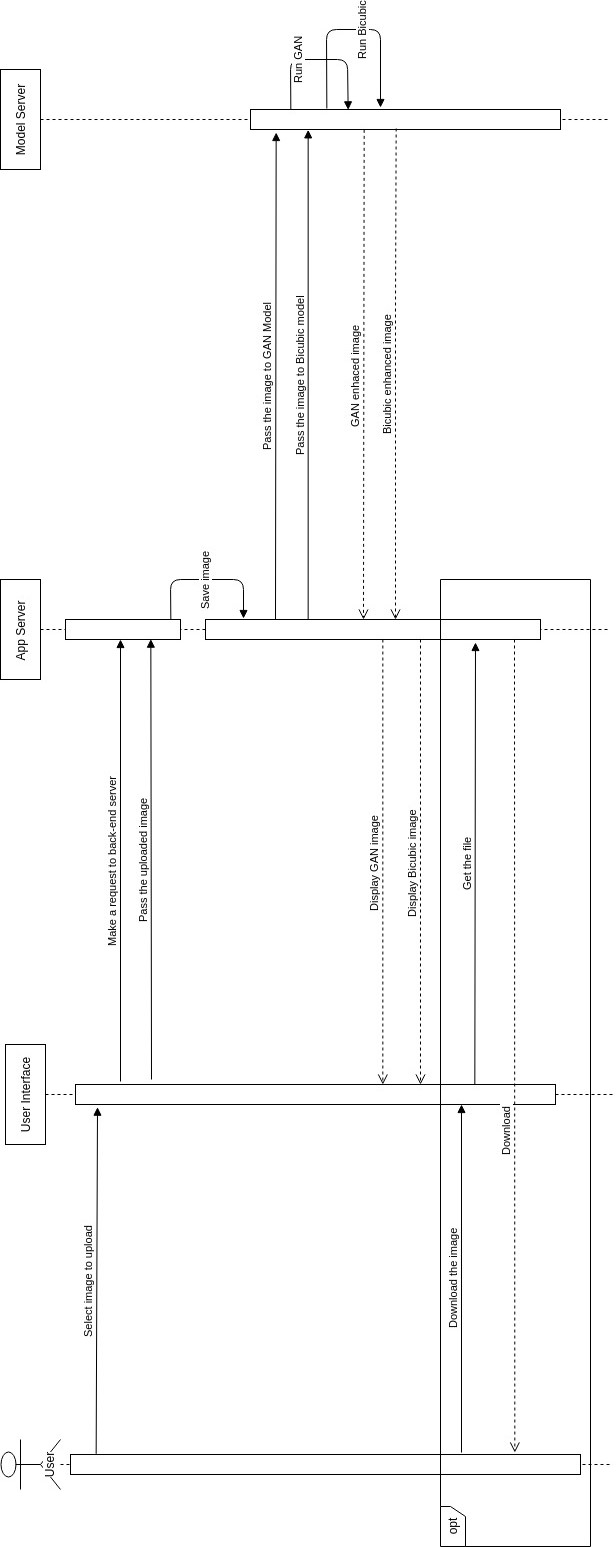
\includegraphics[width=3in]{Images/SequenceDiagram.jpg}
				
					\texttt{Figure 10: Sequence Diagram}
					\vspace{0.1in}
				\end{center}
				\begin{center}
					\vspace{0.1in}
					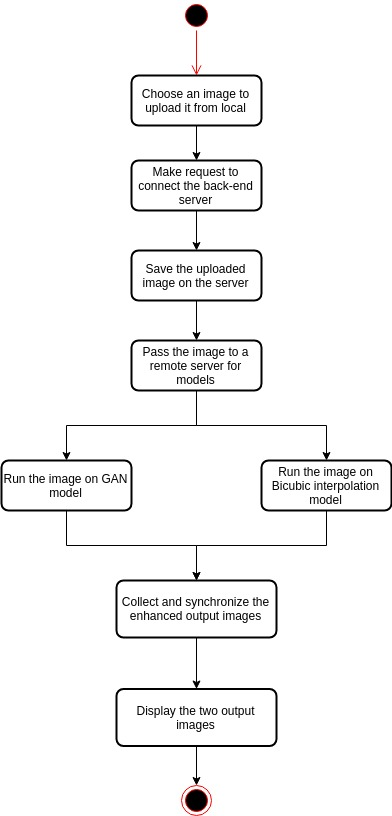
\includegraphics[width=4in]{Images/ActivityDiagram.jpg}
				
					\texttt{Figure 11: Activity Diagram}
					\vspace{0.1in}
				\end{center}
	\section{Evaluation of the Proposed System}
		\subsection{Introduction}
			\textsc{Generative Models}, in particular \textsc{Generative Adversarial Networks} (GANs), have gained significant attention in recent years. A number of GAN variants have been proposed and have been utilized in many applications. Despite large strides in terms of theoretical progress, evaluating and comparing GANs remains a daunting task. While several measures have been introduced, as of yet, there is no consensus as to which measure best captures strengths and limitations of models and should be used for fair model comparison. As in other areas of \textit{Computer Vision} and \textit{Machine Learning}, it is critical to settle on one or few good measures to steer the progress in this field. In this project, we used three main measures for evaluation of enhanced image accuracy to real high-quality image of it. The accuracy measure methods are \textsc{Peak Signal-to-Noise Ratio} (PSNR), \textsc{Structural Similarity Index} (SSIM) and \textsc{Mean Squared Error} (MSE) for fair comparison on images.
		\subsection{Results}
			In this section, we discuss the results of our tested parameters in training in different aspects. We tested the best epoch saved model in different model parameters. Our test was on 500 images from the Flickr2K Dataset \cite{30}, for each model we did the down scaling as the model had trained on, we calculate the average PSNR, SSIM, MSE and Processing Time.
			\begin{center}
				\vspace{0.4in}
				\begin{tabular}{c|c|c|c|c}
					\textbf{Training $I^{HR}$ Resolution} & X & \textbf{256*256} & \textbf{128*128} & \textbf{96*96} \\\hline
					\multirow{2}{*}{\textbf{Average PSNR}} & 2x & -- & 26.73 & 28.15 \\\cline{2-5} & 4x & 21.52 & 21.99 & 22.52\\\hline
					\multirow{2}{*}{\textbf{Average SSIM}} & 2x & -- & 0.76 & 0.85 \\\cline{2-5} & 4x & 0.47 & 0.52 & 0.58\\\hline
					\multirow{2}{*}{\textbf{Average MSE}} & 2x & -- & 181.15 & 163.09 \\\cline{2-5} & 4x & 547.82 & 484.11 & 433.95\\\hline
					\multirow{2}{*}{\textbf{Average Time(sec.)}} & 2x & -- & 0.60 & 2.55 \\\cline{2-5} & 4x & 2.01 & 2.03 & 2.07
				\end{tabular}
				\vspace{0.2in}
					
				\texttt{Table 3: Models Accuracies between different resolutions.}
				\vspace{0.1in}
			\end{center}
			These test were done on the model training machine (i7-8700 CPU, 16 GB RAM, GTX 1080ti GPU).
		\subsection{Evaluation}
			\subsubsection{Mean Squared Error (MSE)}
				In statistics, the \textsc{Mean Squared Error} (MSE) of an estimator measures the average of the squares of the errors. It is the average squared difference between the estimated values and what is estimated. MSE is a risk function, corresponding to the expected value of the squared error loss. The fact that MSE is almost always strictly positive (and not zero) is because of randomness or because the estimator does not account for information that could produce a more accurate estimate. The MSE is a measure of the quality of an estimator, it is always non-negative, and values closer to zero are better.
				
				$$ MSE = \frac{1}{n}\sum_{i = 1}^{n}(Y_i - `Y_i)^2$$
				
				And this is a comparison between our tests:
				\begin{center}
					\vspace{0.1in}
					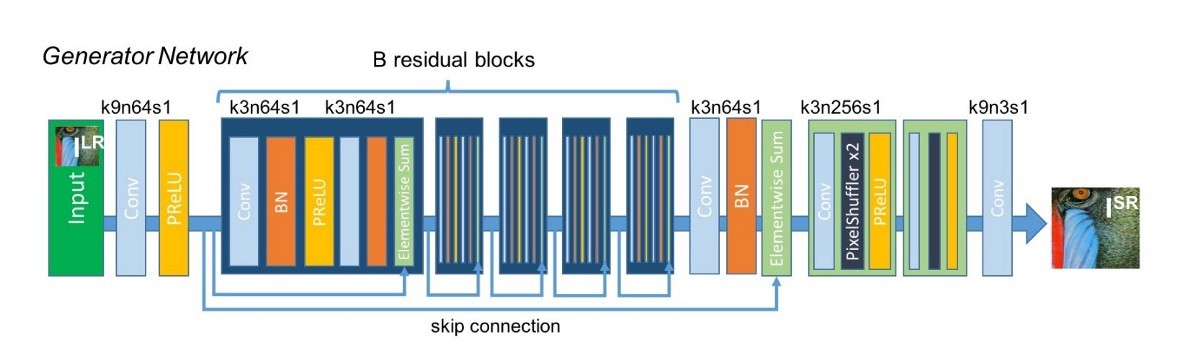
\includegraphics[width=6in]{Images/Generator.jpeg}
				
					\texttt{Figure 12: 4X Models MSE Comparison}
					\vspace{0.1in}
				\end{center}
				\begin{center}
					\vspace{0.1in}
					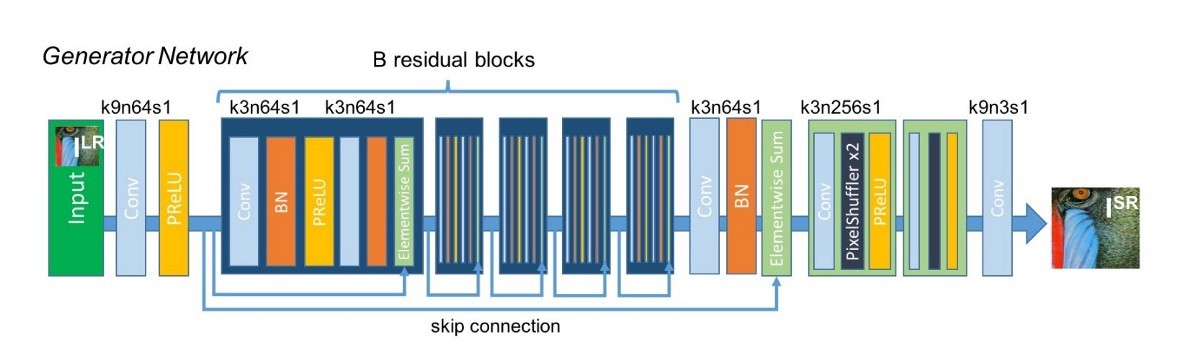
\includegraphics[width=6in]{Images/Generator.jpeg}
				
					\texttt{Figure 13: 2X Models MSE Comparison}
					\vspace{0.1in}
				\end{center}
				\begin{center}
					\vspace{0.1in}
					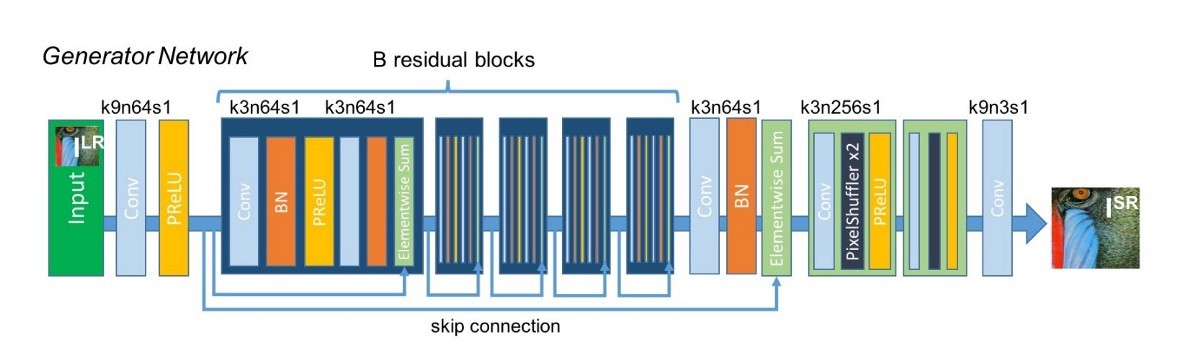
\includegraphics[width=6in]{Images/Generator.jpeg}
				
					\texttt{Figure 13: All Models MSE Comparison}
					\vspace{0.1in}
				\end{center}
			\subsubsection{Peak Signal-to-Noise Ratio (PSNR)}
				\textsc{PSNR} is an engineering term for the ratio between the maximum possible power of a signal and the power of corrupting noise that affects the fidelity of its representation. Because many signals have a very wide dynamic range, PSNR is usually expressed in terms of the logarithmic decibel scale. PSNR is most easily defined via the mean squared error (MSE).
				
				The used equation in our tests for PSNR:
				
				$$ PSNR = 20 * \log_{10}{\frac{MAX_i}{\sqrt{MSE}}} $$
				
				And this is a comparison between our tests:
				\begin{center}
					\vspace{0.1in}
					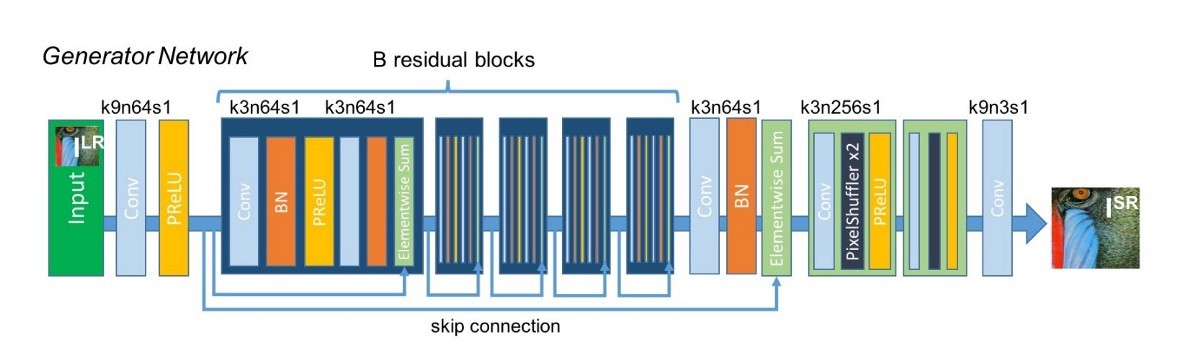
\includegraphics[width=6in]{Images/Generator.jpeg}
				
					\texttt{Figure 14: 4X Models PSNR Comparison}
					\vspace{0.1in}
				\end{center}
				\begin{center}
					\vspace{0.1in}
					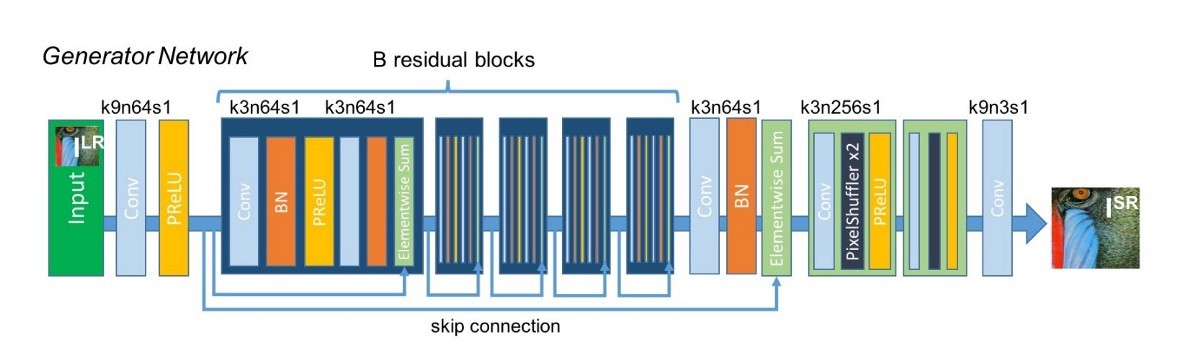
\includegraphics[width=6in]{Images/Generator.jpeg}
				
					\texttt{Figure 15: 4X Models PSNR Comparison}
					\vspace{0.1in}
				\end{center}
				\begin{center}
					\vspace{0.1in}
					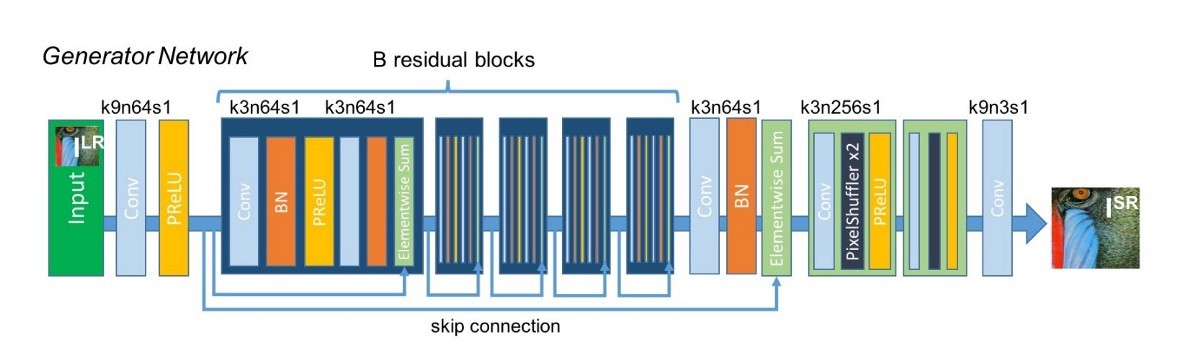
\includegraphics[width=6in]{Images/Generator.jpeg}
				
					\texttt{Figure 15: All Models PSNR Comparison}
					\vspace{0.1in}
				\end{center}
			\subsubsection{Structural Similarity (SSIM)}
				\textsc{SSIM} is a method for predicting the perceived quality of digital television and cinematic pictures, as well as other kinds of digital images and videos. SSIM is used for measuring the similarity between two images. The SSIM index is a full reference metric; in other words, the measurement or prediction of image quality is based on an initial uncompressed or distortion-free image as reference. SSIM is designed to improve on traditional methods such as \textit{Peak Signal-to-Noise Ratio} (PSNR) and \textit{Mean Squared Error} (MSE).
				
				And this is a comparison between our tests:
				\begin{center}
					\vspace{0.1in}
					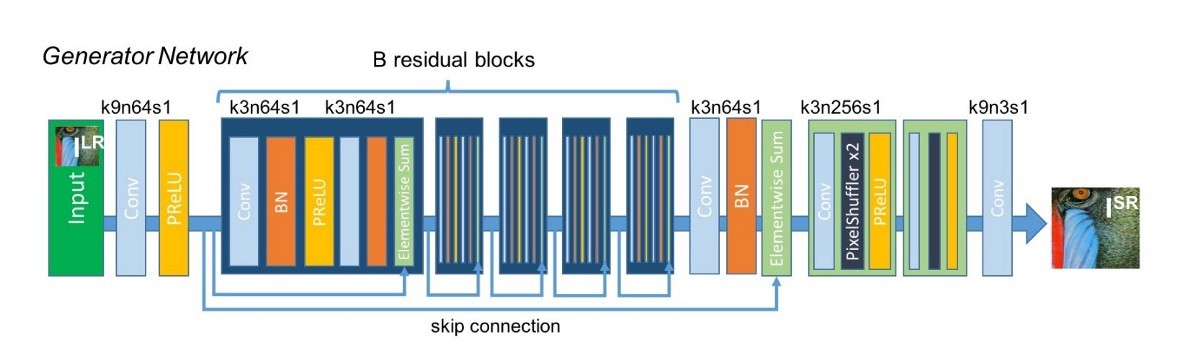
\includegraphics[width=6in]{Images/Generator.jpeg}
				
					\texttt{Figure 16: 4X Models SSIM Comparison}
					\vspace{0.1in}
				\end{center}
				\begin{center}
					\vspace{0.1in}
					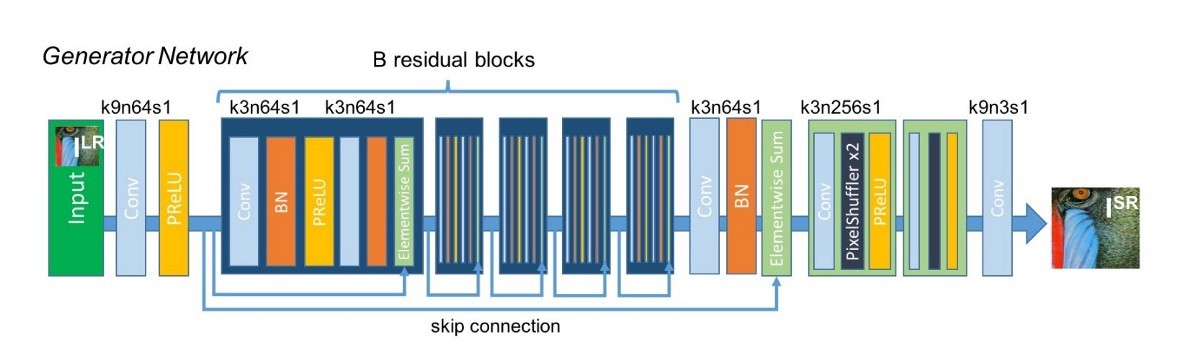
\includegraphics[width=6in]{Images/Generator.jpeg}
				
					\texttt{Figure 17: 4X Models SSIM Comparison}
					\vspace{0.1in}
				\end{center}
				\begin{center}
					\vspace{0.1in}
					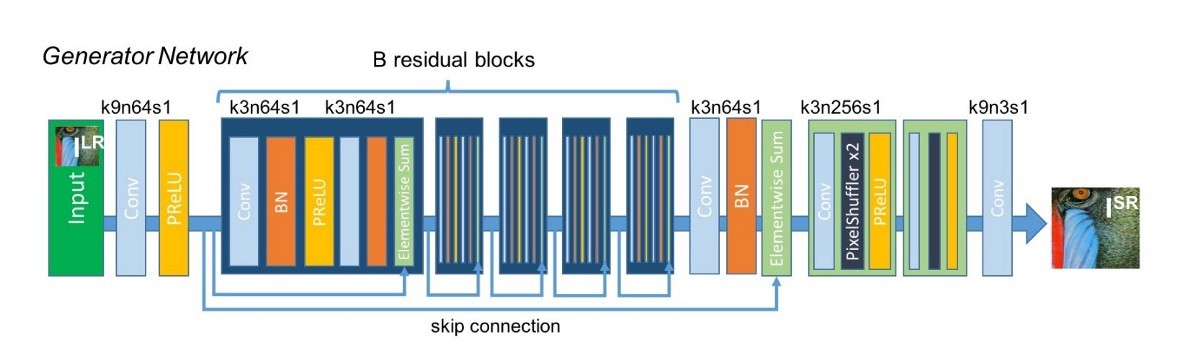
\includegraphics[width=6in]{Images/Generator.jpeg}
				
					\texttt{Figure 17: ALL Models SSIM Comparison}
					\vspace{0.1in}
				\end{center}
	
	\clearpage
	\section{Conclusion}
		We have described a deep residual network Conditional Adversarial Nets of the Generative Adversarial Networks (GAN) model that sets a new state of the art on public benchmark datasets when evaluated with the widely used PSNR measure. We have highlighted some limitations of this PSNR-focused image super-resolution and introduced SRGAN, which augments the content loss function with an adversarial loss by training a GAN. We have confirmed that SRGAN reconstructions for large upscaling factors (4×) are better than traditional image processing techniques and basic neural networks, but close and may be better than GAN models in some cases.
		
	\clearpage
	\begin{thebibliography}{999}
		\bibitem{1} Liang-Jian Deng, Weihong Guo, Ting-Zhu Huang: Single image super-resolution via an iterative reproducing kernel Hilbert space method.
		\bibitem{2} Fattal R. Image upsampling via imposed edge statistics. ACM Transactions on Graphics.
		\bibitem{3} Farsiu S, Robinson MD, Elad M, Milanfar P. Fast and robust multiframe super resolution. IEEE transactions on image processing.
		\bibitem{4} Freeman WT, Pasztor EC. Markov networks for super-resolution. Proceedings of 34th Annual Conference on Information Sciences and Systems.
		\bibitem{5} Sun J, Zheng NN, Tao H, Shum H. Image hallucination with primal sketch priors. IEEE Conference on Computer Vision and Pattern Recognition (CVPR).
		\bibitem{6} Nasrollahi and T. B. Moeslund.  Super-resolution: A comprehensive survey.
		\bibitem{7} C.-Y. Yang, C. Ma, and M.-H. Yang. Single-image super-resolution:A benchmark. InEuropean Conference on Computer Vision (ECCV).
		\bibitem{8} X. Li and M. T. Orchard. New edge-directed interpolation. IEEE Transactions on Image Processing.
		\bibitem{9} W. T. Freeman, T. R. Jones, and E. C. Pasztor. Example-based super-resolution.IEEE Computer Graphics and Applications.
		\bibitem{10} W. T. Freeman, E. C. Pasztor, and O. T. Carmichael. Learning low-level vision.International Journal of Computer Vision.
		\bibitem{11} D. Glasner, S. Bagon, and M. Irani. Super-resolution from a single image. In IEEE  International Conference  on  Computer  Vision(ICCV).
		\bibitem{12} J. B. Huang, A. Singh, and N. Ahuja. Single image super-resolution from transformed self-exemplars. In IEEE Conference on Computer Vision and Pattern Recognition (CVPR).
		\bibitem{13} H. Yue,  X. Sun,  J. Yang, and  F. Wu.Landmark image super-resolution by retrieving web images. IEEE Transactions on Image Processing.
		\bibitem{14} R. Timofte, V. De, and L. Van Gool. Anchored neighborhood regression for fast example-based super-resolution.  In IEEE International Conference on Computer Vision (ICCV).
		\bibitem{15} R. Timofte, V. De Smet, and L. Van Gool. A+: Adjusted anchored neighborhood regression for fast super-resolution.  In Asian Conference on Computer Vision (ACCV).
		\bibitem{16} A. Krizhevsky, I. Sutskever, and G. E. Hinton. Imagenet classification with deep convolutional neural networks. In Advances in Neural Information Processing Systems (NIPS).
		\bibitem{17} K. Simonyan and A. Zisserman. Very deep convolutional networks for large-scale image recognition. In International Conference on Learning Representations (ICLR).
		\bibitem{18} C. Szegedy, W. Liu, Y. Jia, P. Sermanet, S. Reed, D. Anguelov,D. Erhan, V. Vanhoucke, and A. Rabinovich. Going deeper with convolutions. In IEEE Conference on Computer Vision and Pattern Recognition (CVPR).
		\bibitem{19} S. Ioffe and C. Szegedy. Batch normalization: Accelerating deep network training by reducing internal covariate shift. In Proceedings of The 32nd International Conference on Machine Learning (ICML).
		\bibitem{20} J. Kim, J. K. Lee, and K. M. Lee. Deeply-recursive convolutional network for image super-resolution. In IEEE Conference on Com-puter Vision and Pattern Recognition (CVPR).
		\bibitem{21} K. He, X. Zhang, S. Ren, and J. Sun. Deep residual learning for image recognition. In IEEE Conference on Computer Vision and Pattern Recognition (CVPR).
		\bibitem{22} Y. Wang, L. Wang, H. Wang, and P. Li. End-to-End Image Super-Resolution via Deep and Shallow Convolutional Networks.
		\bibitem{23} C. Dong, C. C. Loy, K. He, and X. Tang. Image super-resolution using deep convolutional networks. IEEE Transactions on Pattern Analysis and Machine Intelligence.
		\bibitem{24} X. Yu and F. Porikli. Ultra-resolving face images by discriminative generative networks. In European Conference on Computer Vision(ECCV).
		\bibitem{25} A. Radford, L. Metz, and S. Chintala. Unsupervised representation learning  with  deep convolutional generative adversarial networks.In International Conference on Learning Representations (ICLR).
		\bibitem{26} A. Dosovitskiy and T. Brox. Generating images with perceptual similarity metrics based on deep networks. In Advances in Neural Information Processing Systems(NIPS).
		\bibitem{27} J. Johnson, A. Alahi, and F. Li. Perceptual losses for real-time style transfer and super- resolution. In European Conference on Computer Vision(ECCV).
		\bibitem{28} X. Li and M. T. Orchard. New edge-directed interpolation. IEEE Transactions on Image Processing.
		\bibitem{29} \texttt{https://data.vision.ee.ethz.ch/cvl/DIV2K/}
		\bibitem{30} Jin Yamanaka1, Shigesumi Kuwashima1 and Takio Kurita Fast and Accurate Image Super Resolution by Deep CNN with Skip Connection and Network in Network.
		\bibitem{31} \texttt{cv.snu.ac.kr/research/EDSR/Flickr2K.tar}
	\end{thebibliography}
\end{document}